\documentclass[convert={svg,command=\unexpanded{{inkscape\space --pdf-poppler\space --export-type="svg"\space --pages=1\space -o\space \outfile\space \infile}}}]{standalone}% 'crop' is the default for v1.0, before it was 'preview'

\usepackage{tikz}
\usepackage{pgfplots}
\usepgfplotslibrary{fillbetween}
\usetikzlibrary{patterns, patterns.meta, positioning, math}

\pgfplotsset{compat=1.18}

\usepackage{tikz-3dplot}
\usetikzlibrary{3d}

\pgfplotsset{
	twoDaxis/.style = {
			no marks,
			samples = 100,
			axis lines = center,
			xlabel = {$x$},
			ylabel = {$y$},
			every axis x label/.style={
					at={(ticklabel* cs:1.05)},
					anchor=west,
				},
			every axis y label/.style={
					at={(ticklabel* cs:1.05)},
					anchor=south,
				},
		},
	threeDaxis/.style = {
			axis z line = none,
			axis lines=center, % remove this and you get weird box behavior, not good for calc 2 students
			xlabel=$x$, % you know this one
			every axis x label/.style={
					at={(ticklabel* cs:1.05)},
					anchor=west,
				}, % place the xlabel in a better spot
			ylabel=$y$, % you know this one
			every axis y label/.style={
					at={(ticklabel* cs:1.05)},
					anchor=north,
				}, % places y label in a better spot
		},
	threeDaxiswithyzswap/.style = {
			axis y line = none,
			axis lines=center, % remove this and you get weird box behavior, not good for calc 2 students
			xlabel=$x$, % you know this one
			every axis x label/.style={
					at={(ticklabel* cs:1.05)},
					anchor=west,
				}, % place the xlabel in a better spot
			zlabel=$y$, % you know this one
			every axis z label/.style={
					at={(ticklabel* cs:1.05)},
					anchor=south, % which side of the label gets pinned to the point 5% past the axis end point?
				}, % places y label in a better spot
			xticklabel style = {font=\tiny, yshift=1ex},
			zticklabel style = {font=\tiny, xshift=1ex},
		}
}

\usepackage{tikz-3dplot}
\usetikzlibrary{3d}


\begin{document}
% \tdplotsetmaincoords{45}{37} % Opposite order of pgfplots' view
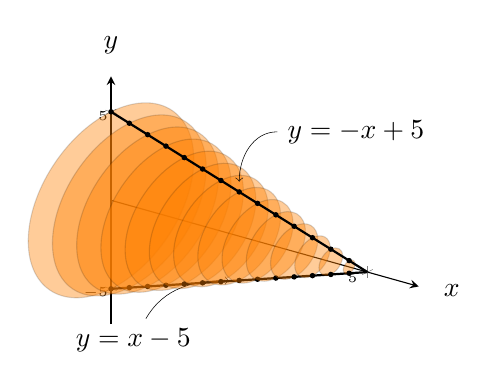
\begin{tikzpicture}[ %tdplot_main_coords,
		area plot/.style={
				fill opacity=0.4,
				draw=black,
				fill=orange,
				mark=none,
				draw opacity = 0.15,
			} % sets up the orange slice fill in stuff
	]
	\begin{axis}[
			view={37}{30}, % first number is how much to rotate around z axis for the view, second is how far above/below you are in angle around x (negative is looking up, positive is looking down)
			axis y line = none,
			axis lines=center, % remove this and you get weird box behavior, not good for calc 2 students
			xlabel=$x$, % you know this one
			every axis x label/.style={
					at={(ticklabel* cs:1.05)},
					anchor=west,
				}, % place the xlabel in a better spot
			zlabel=$y$, % you know this one
			every axis z label/.style={
					at={(ticklabel* cs:1.05)},
					anchor=south, % which side of the label gets pinned to the point 5% past the axis end point?
				}, % places y label in a better spot
			xtick=5, % "generic" type problem so scale on x and y doesn't matter, remove ticks for clarity
			% ytick=\empty,
			xticklabel style = {font=\tiny, yshift=1ex},
			zticklabel style = {font=\tiny, xshift=1ex},
			xmin = 0,
			xmax = 6,
			ymin = -7,
			ymax =  7,
			zmin = -7,
			zmax = 7,
		]
		%plot the curve in the x-y plane, keep "samples y=0" or else, and then just plot coords (x,y,z) like parametric curve sorta where x is the parameter. 
		\addplot3 [black,domain=0:5,samples = 10, samples y=0,thick] (x,0,{x-5}) node [midway, pin={[pin distance=.5cm, pin edge={<-,black, out=180, in=60}]below left:$y=x-5$}] {};
		\tikzmath {
			% set the number of rectangles (it's off by 1 but I don't care)
			\N = 13;
		}
		%set up the loop
		\pgfplotsinvokeforeach{0,...,\N} {
			\tikzmath{
				% calculate the current x value for each iteration (otherwise it acts weird) (the 5 is hard coded the width of theinterval and "#1" is like "i" in a C loop, it is "this iteration number")
				\currentx{#1} = 5/(\N+1)*#1;
				% cacluctate the current y value for each iteration (we use it multiple times so only calculate it once here)
				\currentr{#1} = -1*\currentx{#1}+5;
			}
			\begin{scope}[canvas is yz plane at x = \currentx{#1}]
				\fill[area plot] (0,0) circle (\currentr{#1}cm);
			\end{scope}
			\node [circle,fill,inner sep=0.7pt] at (\currentx{#1},0,\currentr{#1}) {};
			\node [circle,fill,inner sep=0.7pt] at (\currentx{#1},0,-\currentr{#1}) {};
		}
		\addplot3 [black,domain=0:5,samples = 10, samples y=0,thick] (x,0,{-x+5}) node [midway, pin={[pin distance=.5cm, pin edge={<-,black, out=90, in=180}]above right:$y=-x+5$}] {};
	\end{axis}
\end{tikzpicture}
\end{document}
